\section{Applications}
\label{sec:applications}

We investigate two complementary paradigms through which \method enhances general agents.
\method enables infinite environment scaling and controllable simulation~(\S\ref{sec:app:simulator}), allowing agent training to scale to domains and conditions beyond what real environments can provide.
Moreover, LWM training increases the upper bound of downstream agent performance as an agent foundation model~(\S\ref{sec:app:foundation}).

\subsection{Application I: Environment Simulator}
\label{sec:app:simulator}

\begin{tcolorbox}[takeawaysbox]
\small
As a standalone simulator, \method provides \emph{\textcolor{colorscale}{scalability}} and \emph{\textcolor{colorctrl}{controllability}} that real environments cannot offer:
\begin{itemize}[leftmargin=1.2em,itemsep=1pt,topsep=2pt]
\item \textbf{Zero-shot environment generalization.} \method simulates $4k$ OpenClaw environments for agentic RL entirely absent from training, yielding gains of +4.3 on Claw-Eval and +7.1 on QwenClawBench with no domain-specific adaptation.
\item \textbf{Controlled simulation matters.} Controllable perturbations expose agent weaknesses that real-world rarely produce, lifting MCPMark by +12.3 and WideSearch by +16.3, far exceeding uncontrolled Sim RL.
\item \textbf{Surpassing real-environment training.} Controllable Sim RL exceeds Real RL trained using a live search engine (50.3\% vs.\ 45.6\%), while shaping more targeted agent behavior through adversarial snippet design.
\item \textbf{Fictional worlds work.} Agents trained in fully invented, self-consistent worlds generalize to real search tasks, while structurally preventing the agent from confusing simulated facts with real-world knowledge.
\item \textbf{State is the bottleneck.} Sim RL effectiveness depends on providing the world model with a sufficiently detailed initial state; without it, simulation fidelity degrades and downstream gains diminish.
\end{itemize}
\end{tcolorbox}

In this application, \method serves as a standalone environment simulator: the policy agent and the world model are separate models.
\method has two properties that real environments do not provide: \emph{\textcolor{colorscale}{scalability}} (\S\ref{sec:app:scaling}) and \emph{\textcolor{colorctrl}{controllability}} (\S\ref{sec:app:controllable}).

\subsubsection{Generalizable Environment Scaling}
\label{sec:app:scaling}




Leveraging the world knowledge acquired during CPT and the environment modeling capabilities learned across seven training domains, \method can generalizably simulate a wide range of realistic, highly specialized real-world environments.
We study this capability on OpenClaw~\citep{openclaw2026}, an open-source general-purpose real-world AI agent platform whose tasks are drawn from real user multi-step digital workflows rather than curated benchmarks, spanning scheduling, coding, email triage, browser automation, and file management.
Since OpenClaw is entirely out of distribution, it provides a natural testbed for evaluating whether a language world model can generalize to new interactive environment families.
In this setting, \method synthesizes diverse OpenClaw-style environments from a small set of real interaction traces, without any domain-specific adaptation.

\paragraph{Experimental Setup.}
We begin with a small pool of real Claw Agent trajectories as anchors for realistic workflows.
Each trajectory is distilled into a reusable \textbf{seed scenario} that captures the task-relevant \textbf{initial state} (e.g., installed applications, file-system layout, account configuration, and relevant workspace contents) together with the corresponding \textbf{user query}.
From these seeds, we synthesize $4k$ simulated training environments along two complementary axes.
On the environment side, we vary concrete states while preserving the underlying workflow structure; on the task side, we rephrase intents, adjust difficulty, and compose multi-step goals so that the agent sees diverse but realistic OpenClaw-style tasks.
This expansion evaluates the core value of environment scaling: whether a world model can transform scarce real-environment evidence into broad, realistic interaction coverage for downstream agent training.
For each synthesized task, we generate a rubric-based verifier that describes the expected terminal conditions, providing an automatic reward signal for Sim RL.
We use \method-397B-A17B as the simulator to test its generalizable environment simulation capability, with Qwen3.6-Plus as a baseline for ablation.
Based on Qwen3.5-35B-A3B~\citep{qwen35blog}, we conduct multi-turn Sim RL with up to 50 interaction turns and evaluate on Claw-Eval~\citep{ye2026claw} and QwenClawBench~\citep{qwenclawbench}.
For both benchmarks, we report Avg@3 scores with a maximum sequence length of 256k tokens.

\paragraph{Results.}
As shown in Table~\ref{tab:openclaw_simrl}, Sim RL with \method-397B-A17B as the simulator improves the Claw-Eval score from 65.4 to 69.7 (+4.3) and QwenClawBench from 47.9 to 55.0 (+7.1), confirming that \method can scalably simulate a wide range of real-world scenarios and that the resulting policies transfer effectively to real-world domains absent from world-model training.
\textbf{Comparing the two simulators reveals the importance of world-model quality:} using Qwen3.6-Plus as the simulator yields only marginal gains, whereas \method-397B-A17B, trained explicitly for environment simulation, achieves substantially larger gains on both benchmarks, confirming that our dedicated LWM training pipeline is critical for building high-fidelity simulators that produce effective Sim RL gains.


\begin{table}[ht]
\caption{Sim RL on simulated OpenClaw environments. Qwen3.5-35B-A3B is trained via Sim RL using different environment simulators. $\Delta$ reports gains over the base model.}
\label{tab:openclaw_simrl}
\centering
\small
\begin{tabular}{@{}l cc@{}}
\toprule
\textbf{Model} & \textbf{Claw-Eval} & \textbf{QwenClawBench} \\
\midrule
Qwen3.5-35B-A3B          & 65.4 & 47.9 \\
\quad\quad Sim RL~(w/ Qwen3.6-Plus)           & 66.7 & 47.8 \\
\quad\quad Sim RL~(w/ \method-397B-A17B)           & 69.7 & 55.0 \\
\midrule
\quad\quad $\Delta$           & +4.3 & +7.1 \\
\bottomrule
\end{tabular}
\end{table}



\subsubsection{Controllable Simulation}
\label{sec:app:controllable}

Controllable simulation uses natural-language instructions to shape how \method behaves during training, at both the trajectory and turn levels.
Concurrent work on controllable tool-use environments~\citep{xu2026controllable} shares the motivation that oracle-preserving augmentations improve agent robustness.
We validate two complementary modes of controllability via Sim RL on MCP and Search agents respectively.
The base models are Qwen3.5-35B-A3B-SFT and Qwen3.5-397B-A17B-SFT, internal Qwen checkpoints that have undergone continual pre-training and general-purpose supervised fine-tuning but no world-model training:
\begin{itemize}[leftmargin=1.5em,itemsep=2pt]
    \item \textbf{Environment Adaptation}, where the simulator’s behavior and style are adjusted through instructions to inject targeted perturbations, thereby systematically exposing agent weaknesses.
    Control instructions then modify the simulation style and content to produce conditions more extreme or targeted than what real deployments provide, such as intermittent API errors, paginated responses requiring follow-up calls, incomplete intermediate results that force multi-step retrieval, and partial failures in batch operations.
    By systematically exposing the agent to its weak points, controllable Sim RL trains agents that surpass those trained on unperturbed real interactions alone.

    \item \textbf{Fictional-World Construction}, where the simulator generates an entirely fictional environment that is structurally realistic yet factually disjoint from the real world.
    For Search, we instruct \method to simulate a fully fictional, self-consistent world from a compact initial specification.
    LiteResearcher~\citep{li2026literesearcher} independently constructs virtual search worlds for agentic RL with sim-to-real transfer, sharing the same insight that search agents can be trained effectively in simulated environments.
    Fictional-world construction offers two structural advantages for Search-domain Sim RL.
    First, since the answers exist only within the fictional setting, the agent cannot bypass the search tool by answering from parametric memory and must learn to search effectively.
    Second, because all facts are invented with no real-world counterpart, the agent cannot confuse training-time search results with real-world knowledge. By contrast, directly simulating a real search engine risks injecting fabricated but plausible-looking facts that the agent later treats as true.
    \method faithfully follows the initial setting and coherently extends it into a logically consistent reality.
    For instance, a fictional 2030 scenario may specify that 430 people have migrated to Mars.
    The world model then generates consistent demographic records, news articles, and search results grounded in this premise.
    Surprisingly, Search agents trained entirely within these fictional environments generalize effectively to real-world search tasks with significant performance gains.
\end{itemize}

\paragraph{MCP: Environment Adaptation.}
We synthesize environment simulation system prompts from in-house MCP tool-use trajectories collected during the RL data pipeline: frontier agents (Claude Opus 4.6 with extended thinking, DeepSeek-v4-Pro) solve diverse cross-service tasks in real MCP environments, and only trajectories passing automated verification are retained.
Each prompt consists of three components: an \emph{initial state} that specifies the tool schemas and server configuration; an \emph{environment summary} that summarizes the hidden environment state behind the trajectory, such as database contents, permission settings, and service availability; and \emph{controllable simulation instructions} that define how the simulator should respond at each turn, including injected errors, withheld intermediate results, response formats, and the final tool and environment state required for task success.
Together, these components provide the simulator with realistic tool settings, environment context, and clear success criteria.
Since the agent is trained in a simulated environment, a natural concern is whether its gains arise from exploiting simulator-specific artifacts or from ground-truth leakage through the simulation instructions.
However, evaluation on out-of-distribution benchmarks in the real environment eliminates this concern, and the SimRL training data are entirely disjoint from the evaluation queries.
Tool Decathlon~\citep{li2025tool} covers 32 software applications and features multi-step tasks. Performance is measured by execution-verified success rate.
MCPMark~\citep{wu2025mcpmark} evaluates agents on 127 multi-step tasks spanning multiple MCP server categories, using script-verified pass@1 as the metric.

As shown in Table~\ref{tab:controllable_simrl_mcp}, standard Sim RL without control instructions provides no meaningful gain, and Tool Decathlon even drops from 32.4 to 31.5, because the simulator lacks sufficient grounding to produce faithful responses.
With controllable simulation, Tool Decathlon improves by +3.7 and MCPMark by +12.3.
Controllability is not merely a factor in the magnitude of improvement but a prerequisite for Sim RL to work at all in this domain: without grounded simulation instructions, the training signal is too noisy to yield any gain.
The larger gain on MCPMark suggests that controllable simulation is especially effective for tasks that require many tool calls and careful handling of intermediate tool results.


\begin{table}[ht]
\caption{Controllable Sim RL results on Tool Decathlon and MCPMark. ``w/ \method-397B-A17B controlled'' adds targeted environment control instructions during Sim RL.}
\label{tab:controllable_simrl_mcp}
\centering
\small
\setlength{\tabcolsep}{3pt}
\resizebox{\linewidth}{!}{%
\begin{tabular}{@{}l c cccccc c@{}}
\toprule
\multirow{2}{*}[-0.4em]{\textbf{Model}} & \multirow{2}{*}[-0.4em]{\shortstack{\textbf{Tool}\\\textbf{Decathlon}}} & \multicolumn{7}{c}{\textbf{MCPMark}} \\
\cmidrule(lr){3-9}
& & \shortstack{\textbf{Filesys.}} & \shortstack{\textbf{GitHub}} & \shortstack{\textbf{Postgres}} & \shortstack{\textbf{Notion}} & \shortstack{\textbf{Playwright}} & \shortstack{\textbf{WebArena}} & \shortstack{\textbf{Avg.}} \\
\midrule
Qwen3.5-35B-A3B-SFT & 32.4 & 16.7 & 17.4 & 28.6 & 25.0 & 0.0 & 33.3 & 21.5 \\
\quad Sim RL (w/ \method-397B-A17B) & 31.5 & 16.7 & 17.4 & 42.9 & 32.1 & 0.0 & 28.6 & 24.6 \\
\quad Sim RL (w/ \method-397B-A17B controlled) & \textbf{36.1} & \textbf{30.0} & 17.4 & \textbf{47.6} & \textbf{42.9} & 0.0 & \textbf{38.1} & \textbf{33.8} \\
\midrule
\quad $\Delta$ & +3.7 & +13.3 & +0.0 & +19.0 & +17.9 & +0.0 & +4.8 & +12.3 \\
\bottomrule
\end{tabular}%
}
\end{table}

\paragraph{Search: Fictional-World Construction.}
We construct $1k$ self-contained fictional environments using a multi-agent synthesis framework, each anchored by a large relational database (300--500 rows) of internally consistent fictional structured facts.
The pipeline collects high-quality domain documents as grounding material, instantiates fictional database schemas from these documents, populates them via LLM-guided generation, executes SQL to extract ground-truth answers, and reverse-generates natural-language queries.
Four synthesis strategies (time-shifted, granular long-tail, private simulation, realistic grounded) keep the data entirely fictional yet realistic: for instance, a time-shifted environment contains a 2029 smartphone market ranking with real brand names but non-existent model numbers.
Automated retrieval checks and dual rule-based\&LLM validation ensure that synthetic facts conform to real-world patterns (e.g., consistent price ranges, realistic temporal trends) while remaining unsearchable to prevent inject hallucinations.
Controllable simulation instructions further shape \method's turn-level behavior: the world model returns only information relevant to the current search query without revealing the full answer, so the agent must reformulate queries, cross-reference sources, and iteratively aggregate partial results across multiple search rounds.
This design increases the number of tool calls the agent must issue per trajectory, as surface-level search snippets no longer suffice and the agent must invoke page extraction to retrieve complete information (Figure~\ref{fig:sim_vs_real_tool}).
WideSearch~\citep{wong2025widesearch} is a broad information-seeking benchmark of 200 manually curated collection tasks across 15+ domains.
The agent must gather structured tabular answers from the web. The metrics are item-level F1 (per-cell accuracy) and row-level F1 (per-entity completeness).

Table~\ref{tab:controllable_simrl} reports results at both model scales.
On Qwen3.5-35B-A3B-SFT, controllable Sim RL raises F1 by Item from 34.02 to 50.31 (+16.29) and F1 by Row from 13.72 to 24.21 (+10.49).
On Qwen3.5-397B-A17B-SFT, where the base model already achieves 70.11 F1 by Item, Sim RL still yields gains of +3.87 and +6.05 on the two metrics respectively.
These results are notable because the training environments are entirely fictional: every search result, web page, and factual record is invented by \method from scratch, with no connection to any real search engine or real-world database.
The agent never interacts with a real environment during Sim RL, yet the capabilities it acquires (query reformulation, multi-source cross-referencing, and iterative result aggregation) transfer directly to real-world search tasks on WideSearch.
This demonstrates controllability at the level of entire environments: \method constructs and simulates complete, self-consistent fictional worlds that are sufficiently realistic to train effective search agents.
The +16.29 F1 by Item gain at 35B shows that fictional-world Sim RL can close a substantial capability gap for weaker models, while the +3.87 gain at 397B, where the base already achieves 70.11, confirms that the approach remains effective even at frontier scale.

\begin{table}[ht]
\caption{Controllable Sim RL results on WideSearch, using fictional-world simulation.}
\label{tab:controllable_simrl}
\centering
\small
\begin{tabular}{@{}l cc@{}}
\toprule
\multirow{2}{*}{\textbf{Model}} & \multicolumn{2}{c}{\textbf{WideSearch}} \\
\cmidrule(lr){2-3}
& \textbf{F1 Item} & \textbf{F1 Row} \\
\midrule
Qwen3.5-35B-A3B-SFT                          & 34.02 & 13.72 \\
\quad\quad Sim RL (w/ \method controlled) & 50.31 & 24.21 \\
\midrule
\quad\quad $\Delta$                           & +16.29 & +10.49 \\
\midrule
Qwen3.5-397B-A17B-SFT                        & 70.11 & 45.69 \\
\quad\quad Sim RL (w/ \method controlled) & 73.98 & 51.74 \\
\midrule
\quad\quad $\Delta$                           & +3.87 & +6.05 \\
\bottomrule
\end{tabular}
\end{table}


\paragraph{Real RL vs. Sim RL}
The MCP results in Table~\ref{tab:controllable_simrl_mcp} reveal that standard Sim RL without control instructions yields negligible improvement (Tool Decathlon actually drops from 32.4 to 31.5), whereas controlled Sim RL produces substantial gains.
This gap is even more pronounced in the Search domain, where the world model must simulate an entire search engine returning plausible results for fictional facts that no real index contains.
We therefore adopt a fully controllable simulation design from the outset:
the simulation instruction explicitly requires \method to withhold complete answers from search snippets, returning only partial, query-relevant information.
Specifically, snippets are required to \textbf{``tease information without fully answering''}, and each result page mixes highly relevant, moderately relevant, and background results.
This design forces the agent to issue follow-up \texttt{web\_extractor} calls to retrieve full page content rather than relying on surface-level snippets alone.

\begin{figure}[!h]
\centering
\begin{subfigure}[b]{\linewidth}
    \centering
    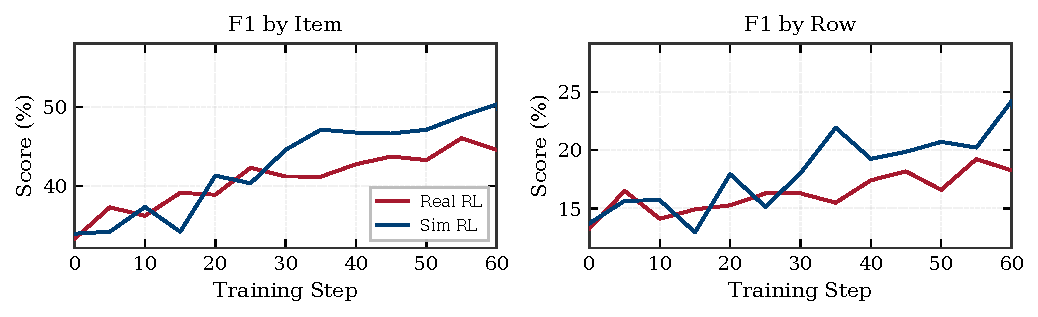
\includegraphics[width=\linewidth]{figures/widesearch_rl_comparison.pdf}
    \caption{F1 by Item and F1 by Row on WideSearch validation set.}
    \label{fig:sim_vs_real_f1}
\end{subfigure}
\\[4pt]
\begin{subfigure}[b]{\linewidth}
    \centering
    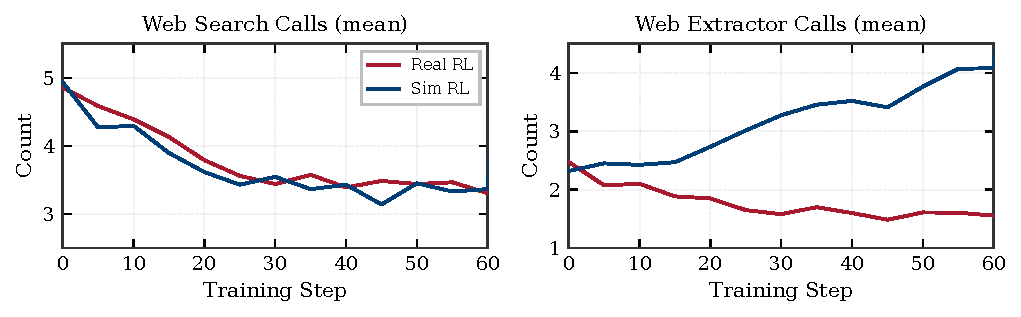
\includegraphics[width=\linewidth]{figures/widesearch_tool_use_comparison.pdf}
    \caption{Mean tool call frequency per trajectory.}
    \label{fig:sim_vs_real_tool}
\end{subfigure}
\caption{Controllable Sim RL vs.\ Real RL (trained against a live search engine) on WideSearch during the first 60 training steps. Both experiments use Qwen3.5-35B-A3B-SFT as the base model.}
\label{fig:sim_vs_real_rl}
\end{figure}

Figure~\ref{fig:sim_vs_real_rl} compares controllable Sim RL against Real RL trained with a live search engine on WideSearch.
In terms of task performance (Figure~\ref{fig:sim_vs_real_f1}), Sim RL tracks or slightly exceeds Real RL throughout the overlapping range: F1 by Item reaches 50.3\%, compared to 45.6\% for Real RL.
\textbf{The more informative signal comes from agent behavior.}
Figure~\ref{fig:sim_vs_real_tool} (left) shows that both training regimes reduce \texttt{web\_search} calls from ${\sim}5$ to ${\sim}3.5$ per trajectory, indicating that both agents learn to issue more targeted queries.
The \texttt{web\_extractor} calls (right), however, diverge sharply: Sim RL increases usage from 2.5 to 4.0 per trajectory, while Real RL decreases it from 2.5 to 1.5.
This divergence directly reflects the controllable simulation design.
Because the simulated search snippets deliberately withhold detailed content, the Sim-RL-trained agent learns that extracting full pages is necessary for assembling complete answers.
In contrast, the Real-RL-trained agent finds that real search snippets often contain sufficient information, and thus learns to skip extraction.
The result confirms that controllable simulation can shape agent behavior in targeted ways: by constructing adversarial environment conditions where specific capabilities are required, Sim RL trains those capabilities more effectively than uncontrolled real-environment training.



\subsection{Application II: Agent Foundation Model}
\label{sec:app:foundation}

\begin{tcolorbox}[takeawaysbox]
\small
LWM training unifies the world model and the agent, instilling next-state prediction as an internalized reasoning capability:
\begin{itemize}[leftmargin=1.2em,itemsep=1pt,topsep=2pt]
\item \textbf{Radical cross-task generalization.} Single-turn, non-agentic LWM RL warm-up with no tool calls transfers to multi-turn, tool-calling agentic tasks across seven benchmarks of five domains.
\item \textbf{Domain generalization.} Gains emerge on two completely out-of-distribution domains entirely absent from LWM training (+11.3 on Claw-Eval, +9.7 on QwenClawBench, and +9.0 on BFCL~v4), confirming transferable capabilities rather than domain-specific shortcuts.
\item \textbf{Next-state prediction as meta-reasoning pattern.} LWM training teaches the agent to mentally simulate environment responses before acting, which generalizes across task formats and domains.
\end{itemize}
\end{tcolorbox}

In Application~I the agent and world model are separate models.
Here we unify them: the same model that selects actions~(agent) also predicts environment states~(world model).
The underlying mechanism is that LWM training enables the agent to mentally simulate the consequences of a candidate action before committing, effectively using world modeling as an internal planning step that improves action quality.
This aligns with the unified \textbf{world-model--actor} architecture envisioned by \citet{lecun2022path} and echoes the \textbf{World Action Model} paradigm emerging in vision-language-action research~\citep{ye2026world}.

LWM RL warm-up familiarizes the agent with how environment states evolve in response to user actions: how different tool calls and search queries yield different responses, which tools are more effective, and how state transitions propagate across turns.
This amounts to learning next-state prediction as a meta-reasoning pattern, in which the agent internally simulates what will happen before deciding what to do.
We validate this effect by running LWM RL on Qwen3.5-35B-A3B-SFT, which is fundamentally a \textbf{single-turn task that involves reasoning with no tool calls or multi-turn interaction} (predicting the next environment state given a user action).
After warm-up, we evaluate the same model directly on \textbf{multi-turn, tool-calling agentic tasks} across seven benchmarks without any additional fine-tuning, including three out-of-domain benchmarks absent from LWM training.
All benchmarks use a maximum sequence length of 256k tokens.
Claw-Eval, QwenClawBench, SWE-Bench Verified, and SWE-Bench Pro scores are averaged over 3 independent rollouts; Terminal-Bench~2.0 scores are averaged over 5 runs; BFCL~v4 uses a single rollout.
SWE-Bench Verified and SWE-Bench Pro are evaluated with an internal agent scaffold (bash and file-edit tools); we correct several problematic tasks in the public set of SWE-Bench Pro and evaluate all baselines on the refined benchmark.
Terminal-Bench~2.0 is evaluated under the Terminus-2 harness with a 3-hour timeout and 8 CPU / 32\,GB RAM.


\begin{table*}[!h]
\caption{Agent foundation model: LWM RL warm-up on single-turn, non-agentic trajectories transfers to multi-turn, tool-calling agentic tasks. No additional fine-tuning is applied after LWM RL.}
\label{tab:foundation}
\centering
\small
\setlength{\tabcolsep}{2.5pt}
\resizebox{\textwidth}{!}{%
\begin{tabular}{@{}l ccc cc c cc ccccccc@{}}
\toprule
& \multicolumn{5}{c}{\textbf{In Domain}} & & \multicolumn{9}{c}{\textbf{Out of Domain}} \\
\cmidrule(lr){2-6} \cmidrule(lr){8-16}
\multirow{2}{*}{\textbf{Model}} & \multirow{2}{*}{\shortstack{\textbf{Terminal-}\\\textbf{Bench 2.0}}} & \multirow{2}{*}{\shortstack{\textbf{SWE-Bench}\\\textbf{Verified}}} & \multirow{2}{*}{\shortstack{\textbf{SWE-Bench}\\\textbf{Pro}}} & \multicolumn{2}{c}{\textbf{WideSearch}} & & \multirow{2}{*}{\shortstack{\textbf{Claw-}\\\textbf{Eval}}} & \multirow{2}{*}{\shortstack{\textbf{QwenClaw}\\\textbf{Bench}}} & \multicolumn{7}{c}{\textbf{BFCL v4}} \\
\cmidrule(lr){5-6} \cmidrule(lr){10-16}
& & & & \textbf{F1 Item} & \textbf{F1 Row} & & & & \textbf{Web} & \textbf{Mem.} & \textbf{Multi-T.} & \textbf{No Live} & \textbf{Live} & \textbf{Hallu.} & \textbf{Avg.} \\
\midrule
Qwen3.5-35B-A3B-SFT & 33.25 & 64.47 & 42.18 & 33.38 & 13.27 & & 53.60 & 39.76 & 67.50 & 54.19 & 47.25 & 78.17 & 77.28 & 82.32 & 62.29 \\
\quad\quad w/ LWM RL & 39.55 & 67.86 & 47.42 & 46.17 & 20.14 & & 64.88 & 49.43 & 83.00 & 60.65 & 60.38 & 80.56 & 79.13 & 84.38 & 71.25 \\
\midrule
\quad\quad $\Delta$   & +6.30 & +3.39 & +5.24 & +12.79 & +6.87 & & +11.28 & +9.67 & +15.50 & +6.46 & +13.13 & +2.39 & +1.85 & +2.06 & +8.96 \\
\bottomrule
\end{tabular}}%
\end{table*}


Table~\ref{tab:foundation} reports the results.
On the four in-domain benchmarks, LWM RL raises WideSearch F1 by Item from 33.38 to 46.17 (+12.79) and F1 by Row from 13.27 to 20.14 (+6.87), Terminal-Bench~2.0~\citep{merrill2026terminal} accuracy from 33.25 to 39.55 (+6.30), SWE-Bench Verified~\citep{jimenez2024swe} resolve rate from 64.5 to 67.9 (+3.4), and SWE-Bench Pro~\citep{deng2025swe} resolve rate from 42.2 to 47.4 (+5.2).
The gains extend to three out-of-domain benchmarks: Claw-Eval~\citep{ye2026claw} improves from 53.6 to 64.9 (+11.3), QwenClawBench~\citep{qwenclawbench} from 39.8 to 49.4 (+9.7), and BFCL~v4~\citep{patil2025berkeley} from 62.3 to 71.3 (+9.0).
The consistent gains across all seven benchmarks are striking.
Even the in-domain results represent a substantial distribution shift: LWM RL trains on single-turn next-state prediction with no tool calls, yet the improvements transfer to multi-turn, tool-calling agentic tasks that require iterative planning, tool selection, and result aggregation, and the benchmark queries are strictly disjoint from LWM training data.
The out-of-domain results demonstrate an even more thorough generalization: the LWM training pipeline contains no Claw or function-calling data whatsoever, yet gains of +11.3, +9.7, and +9.0 emerge on domains entirely absent from world-model training, confirming that LWM warm-up instills transferable agent capabilities rather than domain-specific shortcuts.
Concurrent work by \citet{shrivastava2026echo} provides independent validation from a complementary direction: adding an auxiliary cross-entropy loss on environment observation tokens during agent RL trains the agent to predict terminal outputs as a byproduct of policy optimization, roughly doubling performance on Terminal-Bench~2.0.
This confirms that world-modeling capabilities, whether from dedicated pre-training or auxiliary training signals, consistently transfer to agent performance.
Future work may explore combining LWM warm-up with auxiliary world-modeling objectives during agent training for compounding benefits.




\begin{wrapfigure}{r}{0.4\linewidth}
\centering
\vspace{-4pt}
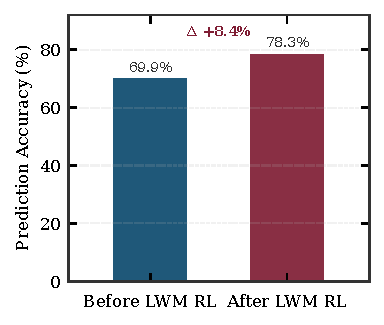
\includegraphics[width=\linewidth]{figures/prediction_accuracy.pdf}
\caption{Environment prediction accuracy on Terminal-Bench 2.0 trajectories.}
\label{fig:prediction-accuracy}
\vspace{-10pt}
\end{wrapfigure}

\paragraph{Insights: Prediction-Driven Action Refinement.}
To understand \emph{why} LWM warm-up transfers to agentic tasks, we examine the reasoning traces produced during multi-turn agentic evaluation.
We find that the RL-trained model systematically performs \textbf{mental simulation} of environment responses before executing actions, using its internalized world model to predict outcomes, identify infeasible approaches, and refine its action plan---all within the thinking trace and before any real execution.

Figure~\ref{fig:case-prediction-refine} illustrates this prediction-driven refinement on the \texttt{mailman} task from Terminal-Bench~2.0, where both models encounter the same Postfix recipient-rejection error.
The model after LWM RL correctly predicts that configuring \texttt{transport\_maps} alone will not work because Postfix rejects unknown recipients \emph{before} consulting transport routing, enabling it to refine its action toward modifying \texttt{local\_recipient\_maps} and apply a targeted fix.
In contrast, the model before LWM RL incorrectly predicts that transport routing precedes recipient validation, preventing productive action refinement and leading to futile exploration before timing out.

To quantify this effect, we first identify interaction turns in which the model's thinking trace contains an explicit prediction of the environment's next state.
For each such turn, we compare the predicted environment response against the actual environment feedback received after execution, and mark the prediction as correct if the two are semantically consistent.
The prediction accuracy is the fraction of correctly predicted turns among all turns that contain an explicit prediction.
Figure~\ref{fig:prediction-accuracy} presents the results.
RL training improves prediction accuracy from 69.9\% to 78.3\% (+8.4\%), confirming that the model's internal world model becomes more faithful through LWM training.
These results provide direct evidence that the performance gains in Table~\ref{tab:foundation} stem from an improved ability to \emph{predict before acting}---a meta-reasoning capability that generalizes across tasks and domains.



\begin{figure*}[t]
\centering
\small
\begin{tcolorbox}[
  colback=gray!3, colframe=black!50, boxrule=0.5pt,
  title={\textbf{Case Study: Accurate Environment Prediction Enables Action Refinement}},
  fonttitle=\bfseries\small, boxrule=0.5pt, arc=2pt
]

\textbf{Task:} \texttt{mailman} --- Configure a Postfix + Mailman3 mailing list server so that emails to \texttt{reading-group-join@local.edu} are routed to Mailman's LMTP service for subscription processing.

\vspace{4pt}
\hrule
\vspace{6pt}

\textbf{Shared Obstacle (both models encounter the same error):}

\vspace{2pt}
\begin{quote}
\ttfamily\scriptsize
\texttt{550 5.1.1 <reading-group-join@local.edu>: Recipient address rejected: User unknown in local recipient table}
\end{quote}

\vspace{2pt}
\noindent Both models configure \texttt{transport\_maps} to route list addresses to Mailman's LMTP (\texttt{lmtp:[127.0.0.1]:8024}). The transport lookup succeeds, yet Postfix still rejects the recipient. Resolving this requires an accurate world model of Postfix's internal processing pipeline.

\vspace{6pt}
\hrule
\vspace{6pt}

\definecolor{casebefore}{HTML}{0c4a6e}
\definecolor{caseafter}{HTML}{7f1d34}
\begin{tcolorbox}[colback=casebefore!5!white, colframe=casebefore, boxrule=0.4pt, arc=1pt, title={\textbf{Before LWM RL}}, fonttitle=\small]

\begin{quote}
\ttfamily\scriptsize
\textcolor{blue!70!black}{[Prediction]} If I configure \texttt{transport\_maps} to route to LMTP, Postfix will\\
use that transport to deliver the mail. The recipient validation against local\\
tables happens \textbf{after} transport routing decides the delivery path.\\
$\Rightarrow$ The transport config should be sufficient. \textcolor{casebefore}{$\times$ Incorrect}\\[4pt]
\textcolor{gray}{[Action] Tries virtual\_alias\_maps, virtual\_transport, relay configs...}\\
\textcolor{gray}{Oscillates between transport\_maps, virtual maps, and relay configurations.}\\
\textcolor{gray}{\textbf{Never modifies local\_recipient\_maps. Task fails (timeout).}}
\end{quote}
\end{tcolorbox}

\vspace{4pt}

\begin{tcolorbox}[colback=caseafter!5!white, colframe=caseafter, boxrule=0.4pt, arc=1pt, title={\textbf{After LWM RL}}, fonttitle=\small]

\begin{quote}
\ttfamily\scriptsize
\textcolor{blue!70!black}{[Prediction]} \texttt{local.edu} is in \texttt{mydestination}. If I only configure\\
\texttt{transport\_maps} without modifying \texttt{local\_recipient\_maps}, Postfix will reject\\
the recipient at the validation stage \textbf{before} transport routing is ever consulted.\\
$\Rightarrow$ The mail will never reach LMTP. \textcolor{caseafter}{$\checkmark$ Correct}\\[4pt]
\textcolor{orange!70!black}{[Refinement]} The fix must target \texttt{local\_recipient\_maps}, not \texttt{transport\_maps}.\\
\hspace{0.5cm} $\rightarrow$ Add Mailman addresses to the local recipient table so they pass validation\\
\hspace{0.5cm} before transport routes them to LMTP.\\[4pt]
\textcolor{teal!80!black}{[Action]} Create \texttt{hash:/var/lib/mailman3/data/local\_recipients} with list addresses. \textcolor{caseafter}{$\checkmark$}\\
\textcolor{gray}{All tests pass.}
\end{quote}
\end{tcolorbox}

\end{tcolorbox}

\caption{Case study of prediction-driven action refinement on the \texttt{mailman} task from Terminal-Bench~2.0.}
\label{fig:case-prediction-refine}
\end{figure*}













